%% -*- TeX-engine: luatex; ispell-dictionary: "russian" -*-

\documentclass[a4paper,12pt]{article}

\usepackage[left=1.5cm,right=2cm,top=1.5cm,bottom=2cm]{geometry}

\usepackage{parskip}
\setlength{\parindent}{0mm}
\setcounter{secnumdepth}{1}

\usepackage{amsmath}

\usepackage{graphicx}

\usepackage{fontspec}
\setmainfont{PT Serif}
\newfontfamily\cyrillicfont[Script=Cyrillic,Ligatures=TeX]{PT Serif}
\setsansfont{PT Sans}
\setmonofont[Ligatures=NoCommon]{PT Mono}
\defaultfontfeatures{Ligatures=TeX}

\usepackage[bold-style=ISO]{unicode-math}
\setmathfont{XITS Math}

\usepackage{microtype}

\usepackage{hyperref}

\usepackage{polyglossia}
\setmainlanguage{russian}
\setotherlanguage{english}

\usepackage{csquotes}

%% for code snippets
\usepackage{minted}
\newminted[pycon]{pycon}{fontsize=\footnotesize}
\newminted[python3]{python3}{fontsize=\footnotesize}
\newminted[bash]{bash}{fontsize=\footnotesize}
\newmintinline[pythoninline]{python3}{fontsize=\footnotesize}
\newmintinline[bashinline]{bash}{fontsize=\footnotesize}

\pagestyle{empty}


\begin{document}
\subsection*{Домашнее задание №8: <<Недвижимость и регрессия>>}

\begin{tabular}{@{}lr}
  \textbf{Дедлайн 1} (20 баллов): &  30 апреля, 23:59 \\
  \textbf{Дедлайн 2} (10 баллов): &  7 мая, 23:59 \\
\end{tabular}

Домашнее задание нужно написать на Python и сдать в виде одного файла.
Правило именования файла: \texttt{name\_surname\_8.[py | ipnb]}. Например, если
вас зовут Иван Петров, то имя файла должно быть: \texttt{ivan\_petrov\_8.py} или \texttt{ivan\_petrov\_8.ipnb}.

\makebox[\linewidth]{\hrulefill}

\begin{figure}[h!]
  \centering
  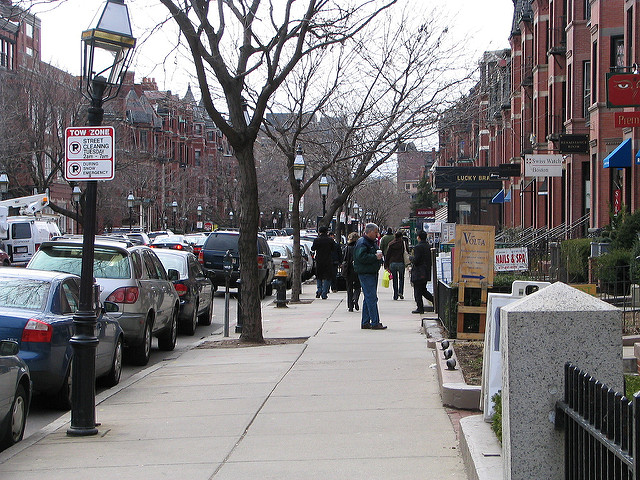
\includegraphics[width=.7\linewidth]{images/houses}
  \caption{Newbury Street, Boston. Источник: \url{https://flickr.com/rudiriet/119512463}}
\end{figure}

Рынок недвижимости в любой стране --- явление непредсказуемое. Цены на жильё
зависят от миллиона факторов, учесть все из которых невозможно, но мы всё-таки
попробуем.

По ссылке%
\footnote{\url{https://gist.github.com/superbobry/1529fb37998d74c6679a}}
находятся данные о стоимости недвижимости в пригородах Бостона. Последняя
колонка каждой строки --- стоимость объекта в долларах. Значения остальных
колонок указаны в заголовке файла.


\paragraph{1} Реализуйте обучение коэффициентов линейной регресии с помощью
нормальной системы уравнений. Структура класса приведена ниже:
\begin{python3}
class NormalLR:
    def fit(self, X, y):
        # ...
        self.weights = weights
        return self

    def predict(self, X):
        # ...
        return y
\end{python3}

При реализации может быть полезно обратиться к пакету \pythoninline{linalg}  \footnote{\url{https://docs.scipy.org/doc/numpy/reference/routines.linalg.html}} из библиотеки \pythoninline{numpy}.

Дополните реализацию методом \pythoninline{predict}, который применяет линейную
регрессию к переданной матрице \pythoninline{X}.

Для отладки алгоритма можно воспользоваться функцией \pythoninline{sample},
порождающей случайную выборку с указанными коэффициентами регрессии.
\begin{python3}
import numpy as np


def sample(size, *, weights):
    X = np.ones((size, 2))
    X[:, 1] = np.random.gamma(4., 2., size)
    y = X.dot(np.asarray(weights))
    y += np.random.normal(0, 1, size)
    return X[:, 1:], y
\end{python3}


С помощью функции \pythoninline{sample} и библиотеки \pythoninline{matplotlib}
можно визуализировать результаты работы алгоритма следующим образом:
\begin{python3}
from matplotlib import pyplot as plt


X, y_true = sample(size, weights=[24., 42.])
lr.fit(X, y_true)
plt.scatter(X, y_true)
plt.plot(X, lr.predict(X), color="red")
plt.show()
\end{python3}


\paragraph{2} Реализуйте метод градиентного спуска для обучения параметров
линейной регрессии. Шаг градиентного спуска:
$$
w^{(t + 1)}_j = w^{(t)}_j
- \frac{\alpha}{l} \sum\limits_{i = 1}^l \left(
      \langle x_i, w^{(t)} \rangle - y_i
  \right) x_{ij}
$$

Убедиться в корректности шага можно, вычислив частные производные по $w_j$ от
функции потерь
$$
Q(w, X^l) = \dfrac{1}{l}
\sum\limits_{i = 1}^l \left( \langle x_i, w \rangle - y_i \right)^2.
$$

Обратите внимание, что в качестве функции потерь используется среднее значение
квадрата ошибки, а не сумма. Такая форма функции потерь удобнее для реализации.

Структура класса приведена ниже:
\begin{python3}
class GradientLR(NormalLR):
    def __init__(self, *, alpha):
        if alpha <= 0:
            raise ValueError("alpha should be positive")
        self.alpha = alpha
        self.threshold = alpha / 100

    def fit(self, X, y):
        # ...
        self.weights = weights
        return self
\end{python3}


\paragraph{3} Реализуйте функцию \pythoninline{mse}, принимающую вектор истинных
значений \pythoninline{y_true} и вектор предсказаний линейной регресии
\pythoninline{y_pred}. Результатом функции является среднее значение квадрата
разности между компонентами векторов.

\paragraph{4} Примените две реализации линейной регрессии к данным, полученным
с помощью функции \pythoninline{sample}. Попробуйте использовать выборки разных
размеров, например, 128, 256, 512, 1024.

Ответьте на вопросы.
\begin{itemize}
\item Какой из подходов имеет меньшее значение средней ошибки?
\item Как ведут себя алгоритмы в зависимости от размера выборки?
\item Что можно сказать о времени работы каждого из алгоритмов?
\end{itemize}

\paragraph{5} Примените две реализации линейной регрессии к данным о стоимости
недвижимости.

Для обучения и оценки следует использовать две различные выборки. Вам может
быть полезна функция \pythoninline{train_test_split} из предыдущего домашнего
задания.

Ответьте на вопросы.
\begin{itemize}
\item Какой из подходов имеет меньшее значение средней ошибки? Согласуется ли
  результат с полученным на симулированных данных?
\item Как вы считаете, требуется ли нормировка признаков в случае данных о
  стоимости недвижимости? Объясните, почему.
\item Интерпретируйте коэффициенты регрессии, полученные одним из
  алгоритмов. Какой из признаков даёт наибольший вклад в стоимость недвижимости?
\item Какой из алгоритмов лучше подходит для задачи предсказания стоимости?
  Почему?
\end{itemize}

\paragraph{6} Модифицируйте оба алгоритма так, чтобы они использовали
регуляризацию весов линейной регресии с помощью $L^2$-нормы. Опишите влияние
регуляризации на значение среднего квадрата ошибки. Как писал классик: <<To
regularize or not to regularize, that is the question [...]>>.


\end{document}
